\section{Statistical inference}

Frequentist inference is hard to understand for lay people. Misunderstandings about \emph{p}-values and confidence intervals are ubiquitous, documented in fields such as psychology \parencite{Belia2005-di,Gigerenzer2018-oi} and medicine \parencite{Goodman2008-ed,Gigerenzer2007-qi}. Frequentist quantities are almost never unique in the same sense as Bayesian quantities, and they are often hard to reason about mathematically. It's easy to forget just how strange hypothesis tests, confidence
sets, and \emph{p}-values are. 

\subsection{Hypothesis tests}

In the following pages, $(\Omega,\mathcal{\mathcal{F}})$ will be a measurable space and $\mathcal{P}$ a background family of probability measures on this space. The family $\mathcal{P}$ contains every probability measure we consider plausible. 
\begin{definition}
\parencite[][Chapter 3.1]{Lehmann2005-sp} Let $\mathcal{P}_{0}$ be a family
of probability measures on $(\Omega,\mathcal{F})$. A test of the
null-hypothesis $P\in\mathcal{P}_{0}$ of \emph{size} $\alpha$ is
a set $R$ such that $\sup_{P\in\mathcal{P}_{0}}P(R)=\alpha.$ A test
of $P\in\mathcal{P}_{0}$ of \emph{level $\alpha$ }is a set $R$
such that $\sup_{P\in\mathcal{P}_{0}}P(R)\leq\alpha.$
\end{definition}

The set $R$ is the \emph{rejection set} of the hypothesis test. Its complement is the acceptance set of the hypothesis and is denoted $A=R^{c}$. The philosophical underpinning of hypothesis test, due to Neyman, is that you have to have make a binary choice. Either you act as if $P\in\mathcal{P}_{0}$ is true, or you act as if $\mathcal{P}_{0}$ isn't true. When you do a hypothesis test, you choose $\mathcal{P}_{0}$ if $\omega\in R^{c}$ and $\mathcal{P}_{1}=\mathcal{P\backslash P}_{0}$, the alternative hypothesis, otherwise. The definition of hypothesis test guarantees you will choose $\mathcal{P}_{1}$ when $\mathcal{P}_{0}$ is true with at most probability $\alpha$. Usually, discussions of hypothesis tests will involve the probability that $\mathcal{P}_{1}$ is chosen when $\mathcal{P}_{1}$ is true; this is called the \emph{power} of the test \parencite{Neyman1977-nx}.

Hypothesis tests are quite easy to understand, especially when formulated with explicit null-hypotheses and alternative hypotheses. The idea behind hypothesis tests is easy to state and has a clear and practical rationale, which is to control error rates. That said, there are examples of even optimal hypothesis tests that behave unintuitively. 

\begin{example}[{\textcite[Example 4a]{Berger1988-ji}}]
 Let $X\in\{1,2,3\}$ and $\theta\in\{1,2\}$. Define
\[
P_{0}(x)=\begin{cases}
0.009, & x=1.\\
0.001, & x=2,\\
0.99, & x=3,
\end{cases},\;P_{1}=\begin{cases}
0.001, & x=1.\\
0.989, & x=2,\\
0.01, & x=3,
\end{cases}
\]
The rejection set $R=\{x\neq3\}$ is the most powerful test of $P_{0}$ vs $P_{1}$, with both error probabilities equal to $0.01$. Now suppose you observe $x=1$, whereupon you would reject $P_{0}$ in favour $P_{1}$ according to $R$. But $x=1$ is $9$ times more likely under $P_{0}$ than under $P_{1}$!
\end{example}

In this example you are you forced to reject $P_0$ since hypothesis test are pre-data constructions. Problems such as these has led to much research into conditional frequentist inference, where conditioning on auxiliary statistics is the best know method. For a review, see \textcite{Goutis1995-ga}.

\subsection{\textit{p}-values}
The complexity goes up a notch with \emph{p-}values.
\begin{definition}
\label{def:p-value}(\textcite[][Chapter 3.3]{Lehmann2005-sp}, \textcite{Bayarri2000-dt}) Let
$A\subseteq[0,1]$ and $R(\alpha)_{\alpha \in A}$ be an increasing sequence of size
$\alpha$ rejection sets under $\mathcal{P}_{0}$, i.e., $R(\alpha')\subseteq R(\alpha)$
when $\alpha'\leq\alpha$, and $\sup_{P\in\mathcal{P}_{0}}P(R)=\alpha$.
Then the random variable
\begin{equation}
U(\omega)=\inf\{\alpha\mid\omega\in R(\alpha)\}\label{eq:size p-value}
\end{equation}
is a \emph{p}-value. 
\end{definition}

Observe that $\{U\leq\alpha\}=\left\{ \omega\mid\inf\{\alpha'\mid\omega\in R(\alpha')\}\leq\alpha\right\}=R(\alpha)$.
Importantly, $U$ satisfies $\sup_{P\in\mathcal{P}_{0}}P(U\leq\alpha)=\sup_{P\in\mathcal{P}_{0}}P(R(\alpha))=\alpha$
for all $\alpha\in A$. When $\mathcal{P}_{0}$ is a singleton, $P(U\leq\alpha)=P(R(\alpha))=\alpha$.
In particular, if $A=[0,1]$, $U$ is uniformly distributed under
$P$, a common definition of a \emph{p}-value in and of itself. The definition
of \emph{p}-value is slightly more general than usual, as it allows
for both $A\neq[0,1]$ and composite hypotheses. The \emph{p}-value
suffers from an all-too-common problem in statistics; there is no
different name for the observed \emph{p}-value $u$ and the \emph{p}-value
statistic $U$. \textcite{Schweder1988-nh} proposed to call $U$ the
``significance statistic'', a name that has unfortunately not caught
on. 

You could claim this definition of a \emph{p}-value is too convoluted. But common definitions of\emph{ p}-values are incomplete, most of them being variants of ``the probability of observing something at least as extreme as the observed data, given the null hypothesis is true.'' A better definition is ``the probability of observing $T\geq t$, where $t$ is a observation of the statistic $T$'', as it makes the dependence on the (often arbitrary) statistic $T$ explicit. But stating the definition in terms of increasing rejection sets is even better, as it makes it clear just how many \emph{p}-values there are, how permissive the definition is, and how the definition is fundamentally about chains of sets in the $\sigma$-algebra $\mathcal{F}$. Moreover, the connection between hypothesis tests and \emph{p}-values is easiest to state and appreciate in terms of rejection sets. For instance, the notion of most powerful \emph{p}-value is obvious; a \emph{p}-value is most powerful against $\mathcal{P}_{1}$ if each rejection set $R(\alpha)$ is a most powerful size $\alpha$ hypothesis test. 

To see why \emph{p}-values should be defined for composite hypothesis, consider the most famous of test of them all, the two-sided $t$-test. The null-hypothesis $\mathcal{P}_{0}$ is the family of normal probabilities with mean zero and any standard deviation $\sigma$, which is composite. Luckily, $\sqrt{n}\overline{x}/s$ is a pivot in this situation, i.e., $P_{\sigma}(\sqrt{n}\overline{x}/s\leq x)$ is independent of $\sigma$, but the null-hypothesis is still composite. The usual formulation hides this though, stating only the insufficient $H_0:\mu = 0$, not $H_0:\mu=0,\sigma>0$.

How should you use \emph{p}-values for inferential purposes? That is really hard to say. A \emph{p}-value does not have the error rate interpretation as an hypothesis test does. And a \textit{p}-value of $0.05$ is not observed with probability $0.05$ under the null-hypothesis, but a \emph{p}-value of $0.05$ or less is observed with probability $0.05$. 

It is demanding to interpret \emph{p}-values. The definition is opaque and hard, if not impossible, to connect to real-life outcomes. And it is hard to justify the use of numbers one cannot expect anyone to interpret in any meaningful way, especially because people will try to interpret it, and inevitably fail. \textcite{Cohen1994-au} wrote, in his critique of \emph{p}-values, 
\begin{quotation}
What's wrong with {[}null-hypothesis significance testing{]}? Well, among many other things, it does not tell us what we want to know, and we so much want to know what we want to know that, out of desperation, we nevertheless believe that it does! What we want to know is \textquotedbl Given these data, what is the probability that $H_{0}$ is true?\textquotedbl{}
\end{quotation}
Some authors, most famously Fisher \parencite{Liu2020-er} attempt to justify \emph{p}-values
as measures of evidence, and, according to \textcite{Berger1987-tf}
most statisticians use \emph{p}-values since they are ``feeling it
to be important to indicate how strong the evidence against $H_{0}$''.
\textcite{Hubbard2008-cg}, among others, are strongly critical of the idea that \emph{p}-values are a measure of evidence, but \textcite{Liu2020-er} defend a slight modification of Definition \ref{def:p-value}, incorporating asymptotic guarantees, as being a reasonable measure of evidence.

One reason why \emph{p}-values are not measures is evidence is the lack of explicit alternative hypotheses. That \emph{p}-values are usually framed without explicit alternative hypotheses is sometimes framed as a strength. \textcite[p. 308]{Barnard1962-rz} wrote that ``the simple tests of significance arise ,it seems to me, in situations where we do not have a parameter space of hypotheses; we have only a single hypothesis essentially, and the sample space then is the only space of variables present in the problem.`` Fisher was firmly against formal alternatives hypotheses and power calculations \parencite{Lehmann1993-oa}. A compelling argument for why alternative hypotheses are important is the Albino argument of \textcite{Berkson1942-hj}:
\begin{quotation}
Suppose I said, \textquotedblleft Albinos are very rare in human populations, only one in fifty thousand. Therefore, if you have taken a random sample of 100 from a population and found in it an albino, the population is not human.\textquotedblright{} This is a similar argument but if it were given, I believe the rational retort would be, \textquotedblleft If the population is not human, what is it?\textquotedblright{} 
\end{quotation}
A major difference between the Neyman--Pearson theory of statistical tests and \textit{p}-values is the theoretical justification. Classical Neyman--Pearson-type inferential statistics, with Lehmann's ``Testing statistical hypotheses'' \parencite{Lehmann2005-sp} as its bible, is concerned with finding optimal tests. Usually, uniformly most powerful tests or uniformly most powerful unbiased tests do not exist, but it is sometimes possible to find other kinds of optimal tests. Optimality theory gives you justification for selecting one test instead of another, and maybe more importantly, forces you to think clearly about exactly what your assumptions are and exactly what you want to test. \emph{p}-values, almost never framed in this way, are much more arbitrary. 

The opaqueness of \textit{p}-values arguably has detrimental consequences for the scientific literature. Since most researchers do not know the definition of \textit{p}-values, much less understand them, they fall back on utterly incorrect ideas about what a \textit{p}-value is or what it entails. Classical examples include \parencite{Gigerenzer2018-oi}:
\begin{itemize}
    \item Replication delusion. The idea that a  \textit{p}-values specifies the probability of a successful replication.
    \item Illusion of certainty. A significant \textit{p}-value proves a purported effect exists.
    \item Bayesian wishful thinking. The \textit{p}-value is the posterior probability of the null-hypothesis being true.
\end{itemize}
\textcite{Gigerenzer2018-oi} found, in a review of the literature comprising a total sample of approximately 1000 academic psychologist and $1000$ psychology students, that $56\% -- 97\%$ of the respondents believed in at least one these incorrect statements. 

Most research follows what \textcite{Gigerenzer2004-oc} calls the \text{null ritual}. The null hypothesis is that of no effect, the \textit{p}-value threshold is $0.05$, and the study is a success if and only if the \textit{p}-value falls below $0.05$. The detrimental effects of this ritual includes \textit{p}-hacking and publication bias, to be discussed in the section about the replication crisis.

\subsection{Confidence sets}
Confidence sets are even harder handle than \emph{p}-values. While
\emph{p}-values are defined in terms of a nested families of rejection
sets, confidence sets need a parameterized families of rejection sets. 
\begin{definition}
\label{def:confidence sets}Let $\Pi=\{\mathcal{P}(\theta)\}_{\theta\in\Theta}$
be a partition of probabilities on a common probability space $(\Omega,\mathcal{F})$.
A confidence set of level $\alpha$ is mapping $R:\Theta\to\mathcal{F}$,
a family of rejection sets, satisfying 
\begin{equation}
\sup_{\theta\in\Theta}\sup_{P\in\mathcal{P}(\theta)}P(R_{\theta})\leq\alpha\label{eq:confidence set}
\end{equation}
If the inequality is an equality, the confidence set has size $\alpha$. 
\end{definition}

Usually we define a set $C(\omega)$ by $\theta\in C(\omega)\iff\omega\notin R_{\theta}$ and call $C$ a confidence set. The definition above uses the well-known duality between rejection sets and confidence sets, and constructing a confidence set from rejection sets in this way is called
\emph{inverting a test}. The definition might look more abstract than necessary, as it involves two suprema. But both are necessary, despite they not showing up in the most familiar examples. The supremum over $\mathcal{P}(\theta)$ guarantees that that $P(R_{\theta})\leq\alpha$
for every $P$ in the equivalence class $\mathcal{P}(\theta)$, while
the supremum over $\Theta$ guarantees that this is the case for each equivalence class.

A confidence set should be regarded as family of rejection sets, not as a random set. For it to be random set we would have to find a $\sigma$-algebra $\mathcal{G}$ over a suitable space of sets $\mathcal{X}$ such that $C:\Omega\to\mathcal{X}$ is measurable, i.e., $C^{-1}(G)\in\mathcal{F}$ for every $G\in\mathcal{G}$. Luckily, this is unneccessary, as we are never interested in questions such a ``What is the probability under $P$ that $C$ is an element of $\mathcal{D}$?''. But a formalization of $C$ as a random set would would be necessary to answer such questions.

Confidence sets are not only hard to define, they are hard to understand. You cannot figure out a handy reformulation of confidence sets, as that does not exist \parencite{Morey2016-ry}. Moreover, confidence sets can be empty; even optimal confidence sets can be empty \parencite[Section 3.1]{Blaker2000-ud}. Well justified confidence set for a real parameter can contain the entire real line \parencite[Section 3.2--3.3]{Blaker2000-ud}. Most confidence sets are asymptotic, but with no guaranteed coverage since uniform convergence almost never is proved, or even true \parencite{Gleser1996-kk}.

\subsection{Impossibility results}

Let's say you have a sequence of real random variables $X_{1},X_{2},\ldots,X_{n}$ from some probability measure $P$ with finite mean $\mu=EX_{1}<\infty$. You do not know anything else about $P$. Is it possible to say anything about the mean $\mu$? From a Bayesian perspective the answer is no, as the problem is underspecified. The problem lacks not only a prior, but a likelihood too. Even worse, there is no $\sigma$-finite dominating measure for the class of candidate $F$s, so Bayes' theorem would be useless in any case. 

But what happens with \emph{p}-values? It turns out there is no nice \emph{p}-value for the mean, or even hypothesis test, for non-parametric families of distributions, even when the variance is finite for every $P$. \textcite{Bahadur1956-tg} proved the following elegant theorem.
\begin{theorem}[Bahadur--Savage]
Let $\mathcal{\mathcal{P}}$ be a family of probability measures
satisfying
\begin{enumerate}
\item[i.)] The expectation $\mu_{F}=\int xdP$ exists and is finite for every
$P\in\mathcal{P}$.
\item[ii.)] For every $\mu\in\mathbb{R}$, there is a $P\in\mathcal{\mathcal{P}}$
satisfying $\mu(P)=\mu$.
\item[iii.)] The family $\mathcal{\mathcal{P}}$ is closed under convex combinations.
That is, if $\lambda\in[0,1]$ and $P,Q\in\mathcal{P}$, then $\lambda P+(1-\lambda)Q\in\mathcal{P}$
too.
\end{enumerate}
Let $\mathcal{P}_{n}(\mu)$ denote the family of probability measures
containing every $P^{n}$ such that $P\in\mathcal{P}$ and $\mu(P)=\mu$.
Let $R$ be a size $\alpha>0$ rejection set for the hypothesis $\mu(P)=\mu_{0}$.
Then 
\[
\sup_{P\in\mathcal{P}_{n}(\mu)}P(R)=\alpha,\quad(\mu\in\mathbb{R})
\]
that is, the maximal probability of rejecting $H_{0}:\mu(P)=\mu_{0}$
is the same for every equivalence class of distributions. In other words,
the test has no uniform power against any alternative hypothesis. 
\end{theorem}

\begin{proof}
Let $R$ be a size $\alpha$ rejection set, in other words, $\sup_{P\in\mathcal{P}_{n}(\mu_{0})}P(R)=\alpha$,
and choose a $\mu\neq\mu_{0}$. Let $\epsilon>0$ be arbitrary and
select a witness $P_{0}\in\mathcal{P}_{n}(\mu_{0})$ satisfying $\alpha\ge P_{0}(R)>\alpha-\epsilon$.
Choose a pair $\lambda,\eta$ such that $\mu=(1-\lambda)\mu_{0}+\lambda\eta$.
Let $P_{\eta}(R)\in\mathcal{P}_{n}(\eta)$ and define $P_{\mu}$ by
$P_{\mu}(A)=(1-\lambda)P_{\mu_{0}}(A)+\lambda P_{\eta}(A).$ When
$A=R$, we obtain the inequality
\begin{eqnarray*}
P_{\mu}(R) & = & (1-\lambda)P_{\mu_{0}}(R)+\lambda P_{\eta}(R),\\
 & \leq & (1-\lambda)\alpha+\lambda.
\end{eqnarray*}
Letting $\lambda\to0$ along with $\eta$, we see that $\sup P_{\mu}(R)\leq\alpha$.
On the other hand,
\begin{eqnarray*}
P_{\mu}(R) & = & (1-\lambda)P_{\mu_{0}}(R)+\lambda P_{\eta}(R),\\
 & \geq & (1-\lambda)(\alpha-\epsilon),
\end{eqnarray*}
hence $\sup P_{\mu}(R)\geq\alpha-\epsilon$ by letting $\lambda\to0$.
Since this is true for every $\epsilon,$ the result follows.
\end{proof}
The Bahadur--Savage theorem tells us that for any sample size $n$, there is no hypothesis test of the mean that has power against a whole class of distributions with any other mean. In a sense, the mean is untestable.

A more recent example of untestable hypothesis testing is \emph{conditional independence testing}. Consider a density with three variables $x,y,z$ and the following test
\begin{align*}
\mathcal{P}_{0}: & p(x,y\mid z)=p(x\mid z)p(y\mid z)\quad\textrm{for all }x,y,z.\\
\mathcal{P}_{1}: & p(x,y\mid z)\neq p(x\mid z)p(y\mid z)\quad\textrm{for some }x,y,z.
\end{align*}
\textcite{Shah2018-jh} proved the following theorem, showing that a
conditional independence test has no power against any alternative. 
\begin{theorem}
\label{theorem:Shah--Peters}Let $n$ be arbitrary and $x_{i},y_{i},z_{i}$ be identically and independently sampled from $P$. Assume $P^{n}(R)\leq\alpha$ for all $P\in\mathcal{P}_{0}$. Then $P^{n}(R)\leq\alpha$ for all $P\in\mathcal{P}_{1}$ too.
\end{theorem}

The Shah--Peters theorem is stronger than the Bahadur--Savage theorem in the sense its alternatives are simple, not composite. The alternatives in Bahadur--Savage are entire classes of probability measures; and the richness of these classes is what drives the theorem. The Shah--Peters theorem, on the other hand, is about the richness of the the null hypothesis, $\mathcal{P}_{0}$. This class of distributions is so large that any rejection set satisfying $P^{n}(R)\leq\alpha$ for all $P\in\mathcal{P}_{0}$ must satisfy $P^{n}(R)\leq\alpha$ for all $P\in\mathcal{P}_{1}$ too.

An analogue of the Shah--Peters result does not hold for unconditional independence testing, as the rank test of \textcite{Hoeffding1948-nm} test is pointwise consistent. Still, there is no uniformly unbiased test of independence \parencite{Moss2020-bc}.

\textcite{Donoho1988-hg} studies conditions when two-sided confidence intervals fail to exist, but one-sided do. Consider the problem of estimating the number of modes in a continuous density. If we make no assumptions about the shape of the density, such as smoothness assumptions of various kinds, it is impossible to put an upper bound on its number of modes. The intuition here is simple, as illustrated in Figure \ref{fig:donoho}. You might be able to identify "large" modes from limited data, but you will not be able to identify the "small" ones. But Donoho proved there is possible to find lower bounds for the number of nodes, hence it is possible to construct a one-sided confidence interval for the number of modes in a non-parametric density.

\begin{figure}
    \centering
    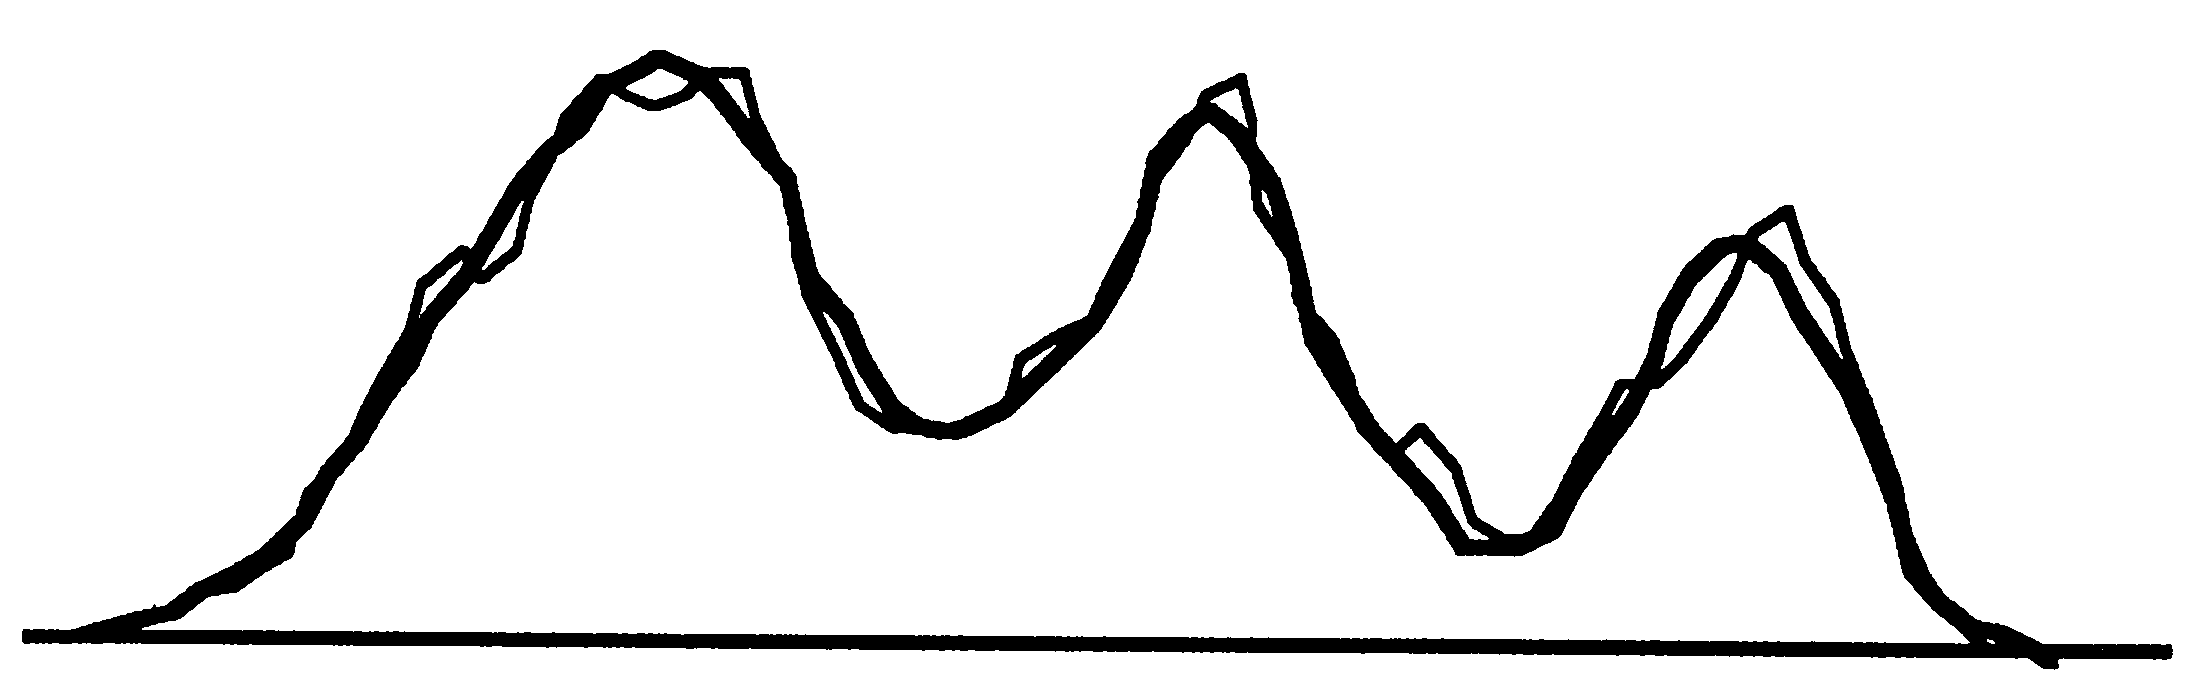
\includegraphics[scale=0.16]{chunks/donoho.png}
    \caption{Thick line: a density with three modes. Thin line: The same density pertubed to have three modes. Taken from the paper of \textcite{Donoho1988-hg}.}
    \label{fig:donoho}
\end{figure}

The mean of normal model with known standard deviation is connected to three confidence intervals. The standard two-sided, the left-sided, and the right-sided. In this case, the two-sided confidence interval will always have finite diameter, or length, while the left-sided and right-sided will always have infinite diameter. But there are models and parameters where there is no confidence interval of guaranteed finite length. \textcite{Gleser1987-ii} proved a beautiful theorem giving sufficient conditions for there to be no confidence interval of guaranteed finite diameter. Essentially, if there is a sequence $\theta_n$ of parameters such that $|\theta_n| \to \infty$ while $f_{\theta_n} \to f$ for some density $f$, then there is no confidence interval for $\theta$ of guaranteed finite diameter. A simple example is $\theta = 1/\mu$, where $\mu$ is the mean of a normally distributed variable with fixed standard deviation. For in this case, $\mu_n = 1/n$ implies $\theta_n\to\infty$, while the density $f_\mu$ converges to a standard normal.